\documentclass[]{article}
\usepackage{geometry}
 \geometry{
 a4paper,
 total={170mm,257mm},
 left=20mm,
 top=20mm,
 }
\usepackage{graphicx}
\usepackage{subcaption}
\usepackage{listings}
\usepackage[justification=centering]{caption}
\usepackage[hidelinks]{hyperref}
\usepackage{enumitem}
\usepackage[utf8]{inputenc}
\usepackage{float}
\DeclareTextFontCommand{\helvetica}{\fontfamily{phv}\selectfont}
\setlength{\parindent}{4em}
\setlength{\parskip}{1em}
\linespread{1.5}

\usepackage[table]{xcolor}
\usepackage{graphicx}


\title{PAC2  Desenvolupament el treball - Fase 1}
\date{18 de Març 2019}
\author{Vasyl Druchkiv \\ Estudiant de Màster de Bioestadística i Bioinformàtica}
\renewcommand{\contentsname}{Índice}
\usepackage{setspace}


\renewcommand\paragraph{\@startsection{paragraph}{4}{\z@}%
            {-2.5ex\@plus -1ex \@minus -.25ex}%
            {1.25ex \@plus .25ex}%
            {\normalfont\normalsize\bfseries}}

\begin{document}
\maketitle
\makeatletter

\makeatother
\begin{spacing}{0.1}
\tableofcontents
\end{spacing}



    \section{Identificació del treball i data de l'informe}

    \section{Descripció de l'avanç del projecte} 

A la data d'avui he desenvolpupat l'aplicació d'anàlisis de les rutes. L'aplicació es completament funcional localment i ofereix l'anàlisi a partir de les bases de dedes GO, KEGG i Reactome. Com estava previst, l'usuari indica l'especie, puja l'arxiu amb els gens i els LogRatios provenents d'estudi de microarrays o NGS. 

L'aplicació està dividira doncs en 4 parts substancials:

\begin{enumerate}
\item Entrada de les dades;
\item Anàlisi GO;
\item Anàlisi KEGG;
\item Anàlisi Reactome.
\end{enumerate}

\begin{figure}[h!]
\caption{Pàgina d'entrada}
\centering
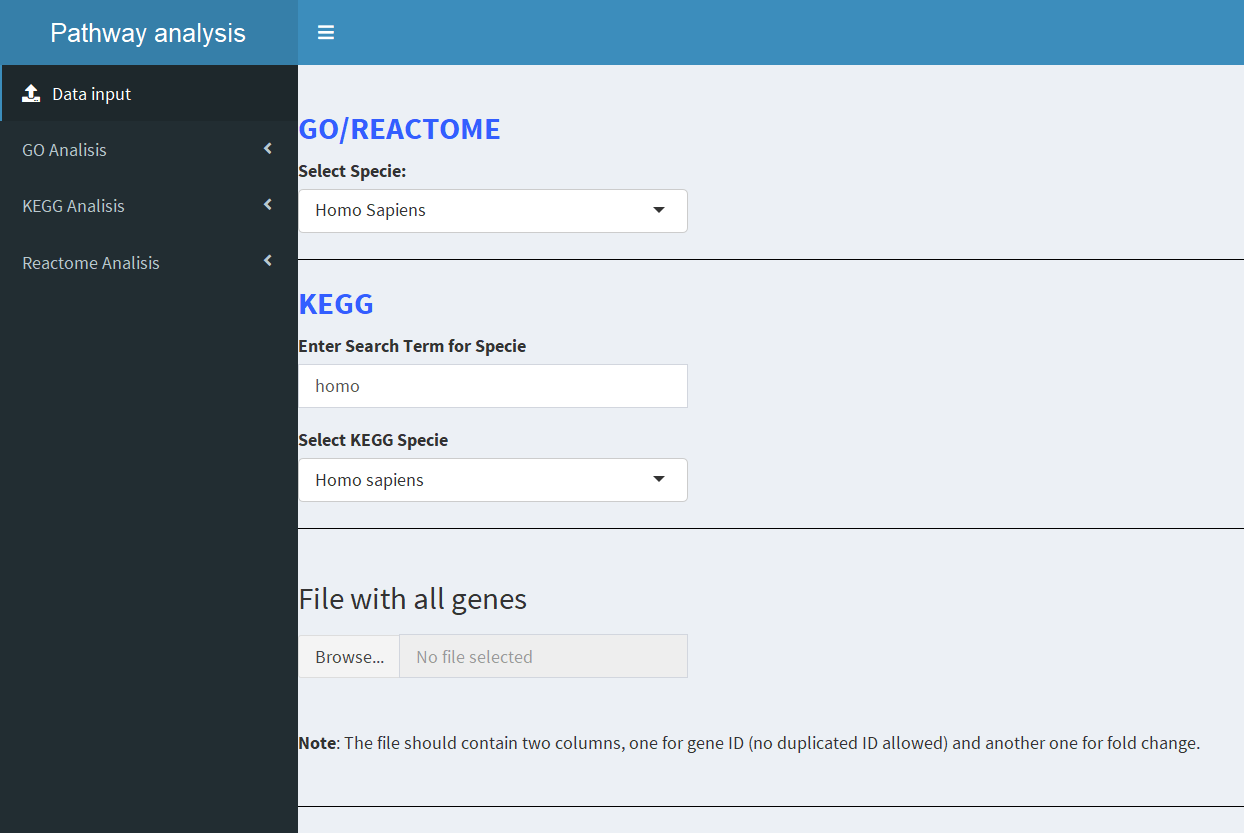
\includegraphics[width=0.9\textwidth]{App_F1}
\end{figure}

L'aplicació ofereix dos mètodes d'anàlisi: d'una banda es pot  fer ORA (Over-Representation Analysis) i d'altra banda l'anàlisi GSEA (Gene Set Enrichment Analisis). Recordem que l'ORA consisteix en selecionar els gens diferencialment expressats i basant-se en GO, KEGG o Reactome comprobar si una de les agrupacións de gens suggerides per aquestes bases de dades està sobre o sotraexpressada en els gens selecionats. Per dur a terme l'ORA l'usuari té opció de definir un \textit{cut-off} de Log-Ratio per formal el conjunt dels gens que s'hi utilitzara (\textit{gene set}). ORA és una bona eina per veure els efectes grans però els effectes petits li escapen.  Els efectes petits derivats dels gens individuals poden acommular-se en un efect conjunt substancial el qual ORA no serà capaç de detectar. És aquí on GSEA mostra la seva utilitat. 

Els apartats d'anàlisi (GO, KEGG i Reactome) ofereixen tan representacions comunes com representacions específiques. 

Els anàlisis i representacions  \underline{en comú} són:

\begin{itemize}
\item Taula dels resultats ORA;
\item Taula dels resultats GSEA;
\item Gràfic de barres del resultat ORA;
\item Gràfic de punts del resultat ORA;
\item El mapa d'enriquement (Enrichment Map);
\item La red dels gens en categories (Category-gene-network);
\item El gràfic lde GSEA.
\end{itemize} 

Els anàlisis \underline{específics} són:

\begin{itemize}
\item GO $\rightarrow$ Gràfic GO 
\item KEGG $\rightarrow$ Rutes de la base de dades KEGG
\item Reactome $\rightarrow$ Rutes de la base de dades Reactome
\end{itemize}

\begin{figure}[h!]
\centering
\begin{tabular}{ccc}
  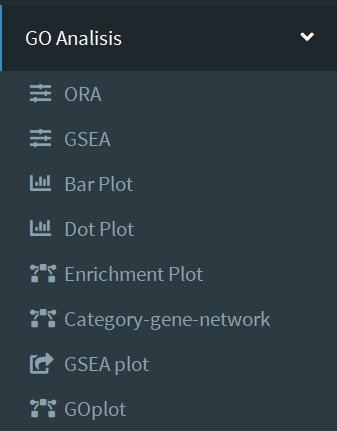
\includegraphics[width=45mm]{App_F2_Items_GO.png} &   
  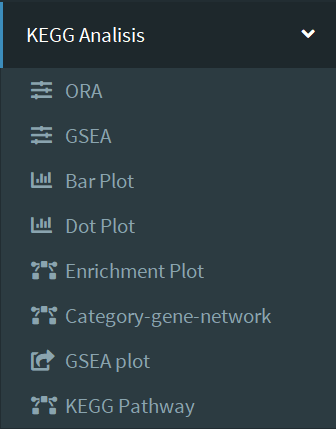
\includegraphics[width=45mm]{App_F3_Items_KEGG.png} &
  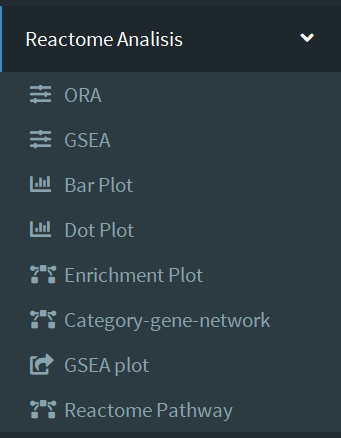
\includegraphics[width=45mm]{App_F4_Items_RA.png} \\
(a) GO & (b) KEGG & (c) Reactome \\
\end{tabular}
\caption{Els elements de les seccions d'anàlisi}
\end{figure}

\section{L'anàlisi comú de GO, KEGG i Reactome}

\subsection{ORA}

\subsubsection{GO}

Per realitzar l'anàlisi ORA per a termes GO s'utilitza la funciió \helvetica{enrichGO} del paquet \helvetica{clusterPrifiler}.
\begin{lstlisting}[language=R]
enrichGO(gene, OrgDb, keyType = "ENTREZID", ont = "MF", pvalueCutoff = 0.05, 
pAdjustMethod = "BH", universe,  qvalueCutoff = 0.2, minGSSize = 10, maxGSSize = 500,  
readable = FALSE, pool = FALSE)
\end{lstlisting}

He implementat els valors per defecte amb la possibilitat per a usuari d'ellegir entre:

\begin{itemize}
\item \underline{Ontologies GO} 
\begin{itemize}
\item Molecular function, Biological proces, Cellular Components;
\end{itemize}
\item \underline{Nivell de significació basant-se en els valors de P ajustats}
\begin{itemize}
\item 0.1, 0.05, 0.01, 0.001;
\end{itemize}
\item \underline{Mètode d'ajustament}
\begin{itemize}
\item Holm; Hochberg; Hommel; Bonferroni; BH; BY; FDR; None.
\end{itemize}
\end{itemize}

\begin{figure}[h!]
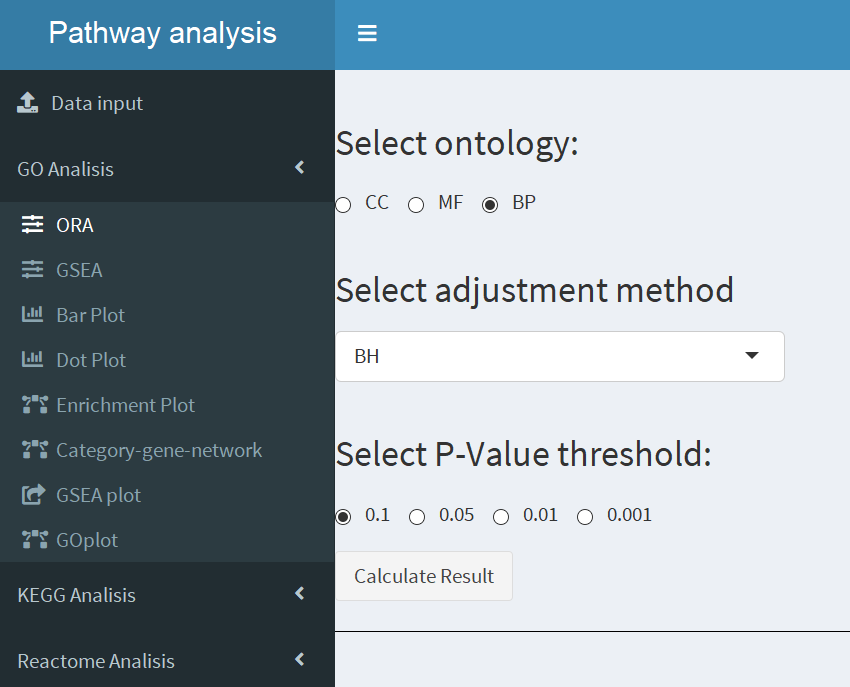
\includegraphics[width=0.9\textwidth]{App_F5_Items_GO_ORA.png}
\caption{Especificació d'ORA dels termes GO}
\end{figure}
L'execució de la funció és un procès temporalment costòs. Per aquest motiu he afegit el botó d'acció, en lloc de deixar la funció reactiu.  D'aquesta manera l'usuari ha de fer una decisió consient de repetir l'anàlisi amb altres valors.

Apretant el botò apareix la taula i el botò nou mitjançant el qual l'usuari pot descargar els resultats en format .csv. He formateat la taula amb els paquets \helvetica{knitr}, \helvetica{kableExtra},  \helvetica{formattable} i \helvetica{dplyr}. Amb els dos últims he afegit les barres de color per el nombre dels gens diferencialment expressats del terme específic de GO i el gradient de color del verd fins vermell pels valors de més petits fins els més grans. 

\begin{figure}[h!]
\centering
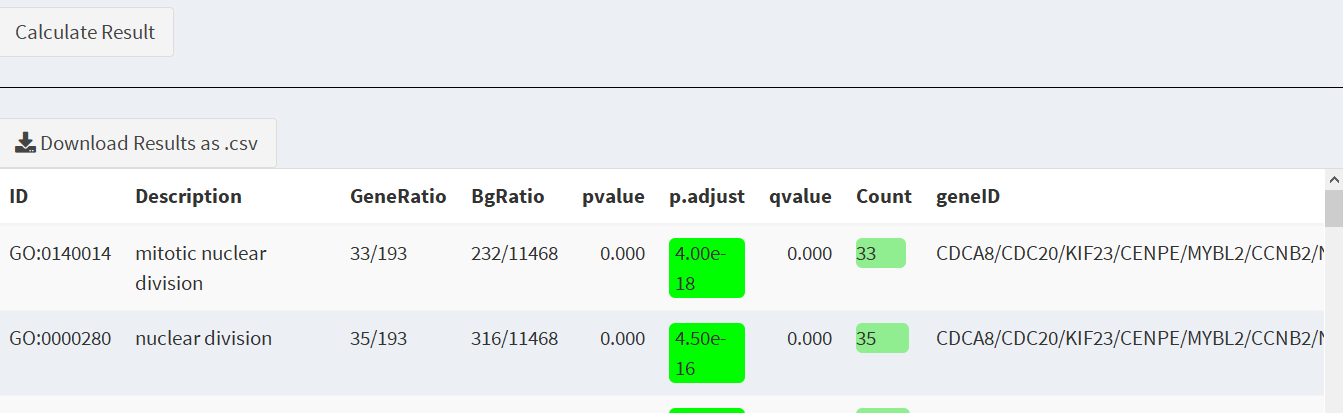
\includegraphics[width=0.9\textwidth]{App_F6_Items_GO_ORA_Table.png}  
\caption{El resultat d'anàlisi ORA. GO.}
\end{figure}

Els camps més interesants de la taula són:

\begin{itemize}
\item \underline{Description}. El nom del terme GO;
\item \underline{GeneRatio}. El quotient: $\displaystyle\frac{\mbox{Nombre dels gens diferencialment expressats}}{\mbox{Nombre total dels gens en la mostra}}$; 
\item \underline{BgRatio}. El quotient: $\displaystyle\frac{\mbox{Nombre dels gens de la ruta}}{\mbox{Nombre total dels gens en la base de dades GO}}$;
\item \underline{p.adjust}. El valor de P ajustat.
\end{itemize}

\subsubsection{KEGG}

Per l'ORA de base de dades KEGG he utilitzat la funció \helvetica{enrichKEGG()} del paquet \helvetica{clusterProfiler}.  

\begin{lstlisting}[language=R]
enrichKEGG(gene, organism = "hsa", keyType = "kegg", pvalueCutoff = 0.05, 
pAdjustMethod = "BH", universe, minGSSize = 10, maxGSSize = 500, 
qvalueCutoff = 0.2, use_internal_data = FALSE)
\end{lstlisting}

Com en el cas de l'anàlisi dels termes GO també aquí l'usuari té la llibertat d'elegir  l'organisme, el \textit{cut-off} del valor de P i el mètode d'ajustament. Perquè la funció necessita el codi kegg', 'ncbi-geneid', 'ncib-proteinid' o 'uniprot' l'usuari ha d'especificar altra vegada l'especie. La llista de les especies disponibles per a anàlisi de KEGG és molt llarga. Per aquest motiu he abilitat l'eina de cerca d'espècie per a usuari.

\begin{figure}[H]
\centering
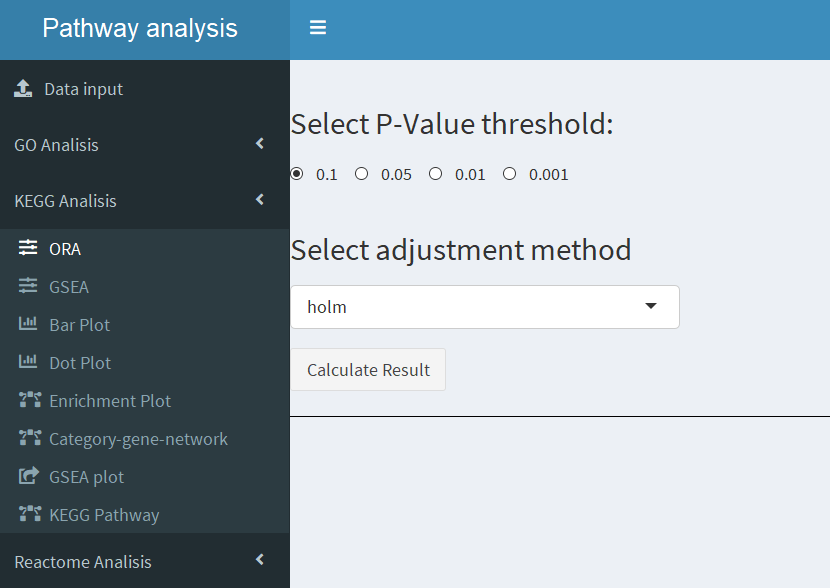
\includegraphics[width=0.9\textwidth]{App_F7_Items_KEGG_ORA.png}  
\caption{El resultat d'anàlisi ORA. KEGG.}
\end{figure}

\begin{figure}[H]
\centering
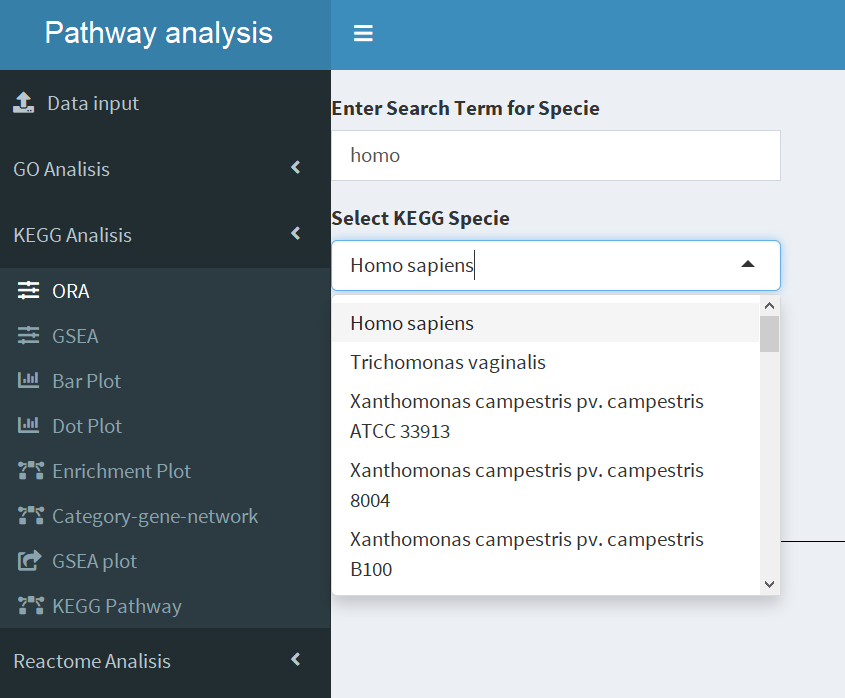
\includegraphics[width=0.9\textwidth]{App_F8_Items_KEGG_ORA_Search.png}  
\caption{L'eina de cerca d'espècie. KEGG.}
\end{figure}

Una vegada introduïts els paràmetres i apretat el botó \textbf{Calculate} apareix el botó \textbf{Download .csv} i la taula previsualitzada. Els camps de la taula són els mateixos com d'anàlisi dels termes GO.
 
\begin{figure}[H]
\centering
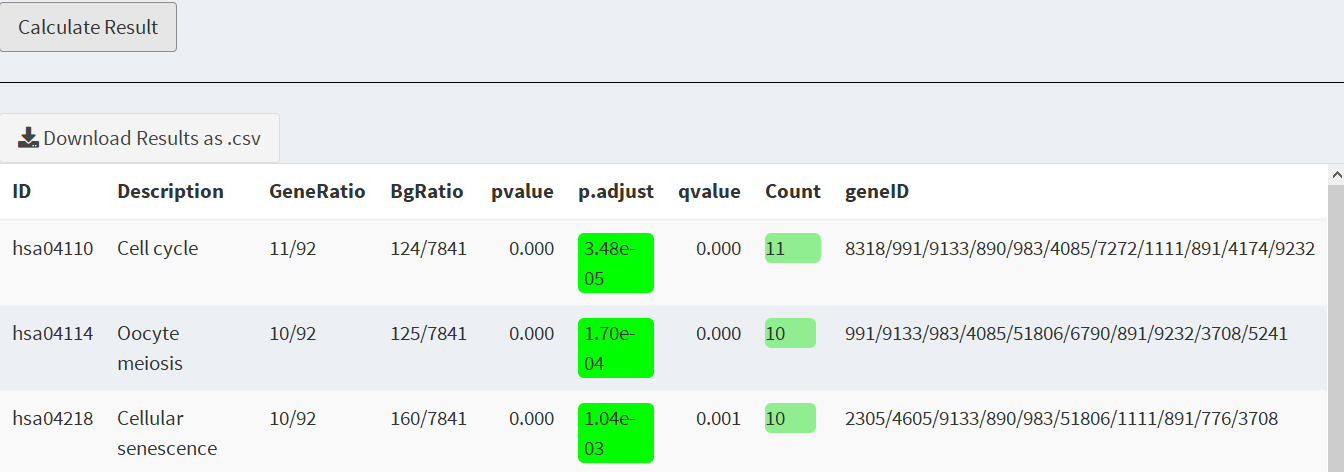
\includegraphics[width=0.9\textwidth]{App_F9_Items_KEGG_ORA_Table.png}  
\caption{El resultat d'anàlisi ORA. KEGG.}
\end{figure}

\subsubsection{Reactome}
Al cas de Reactome el procediment és similar. La funció usada és \helvetica{enrichPathway()} del paquet \helvetica{ReactomePA}:

\begin{lstlisting}[language=R]
enrichPathway(gene, organism = "human", pvalueCutoff = 0.05,
  pAdjustMethod = "BH", qvalueCutoff = 0.2, universe, minGSSize = 10,
  maxGSSize = 500, readable = FALSE)
\end{lstlisting}

Aquí l'usuari ha de seleccionar l'altra vegada l'organisme. Les opcions disponibles són: "human", "rat", "mouse", "celegans", "yeast", "zebrafish", "fly".

\begin{figure}[H]
\centering
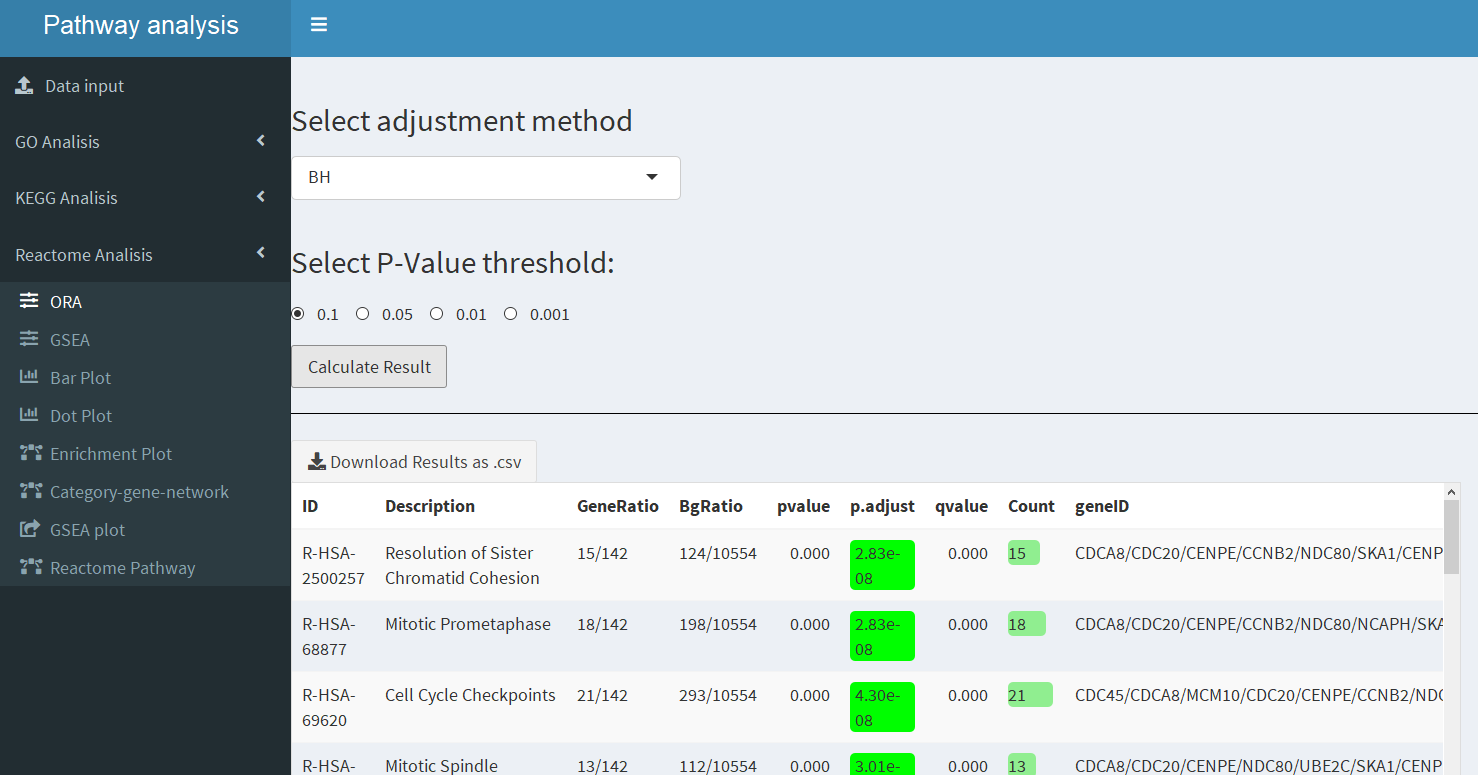
\includegraphics[width=0.9\textwidth]{App_F10_Items_Reactome_ORA.png}  
\caption{El resultat d'anàlisi ORA. Reactome.}
\end{figure}

\subsection{GSEA}
\subsubsection{GO}
El mètode GSEA per a termes GO es calcula amb la funció \helvetica{gseGO()} del paquet \helvetica{clusterProfiler}. 

\begin{lstlisting}[language=R]
gseGO(geneList, ont = "BP", OrgDb, keyType = "ENTREZID",
  exponent = 1, nPerm = 1000, minGSSize = 10, maxGSSize = 500,
  pvalueCutoff = 0.05, pAdjustMethod = "BH", verbose = TRUE,
  seed = FALSE, by = "fgsea")
\end{lstlisting}

L'usuari pot elegir l'ontologia GO, el \textit{cut-off} del valor P i el mètode d'ajustament.
\begin{figure}[H]
\centering
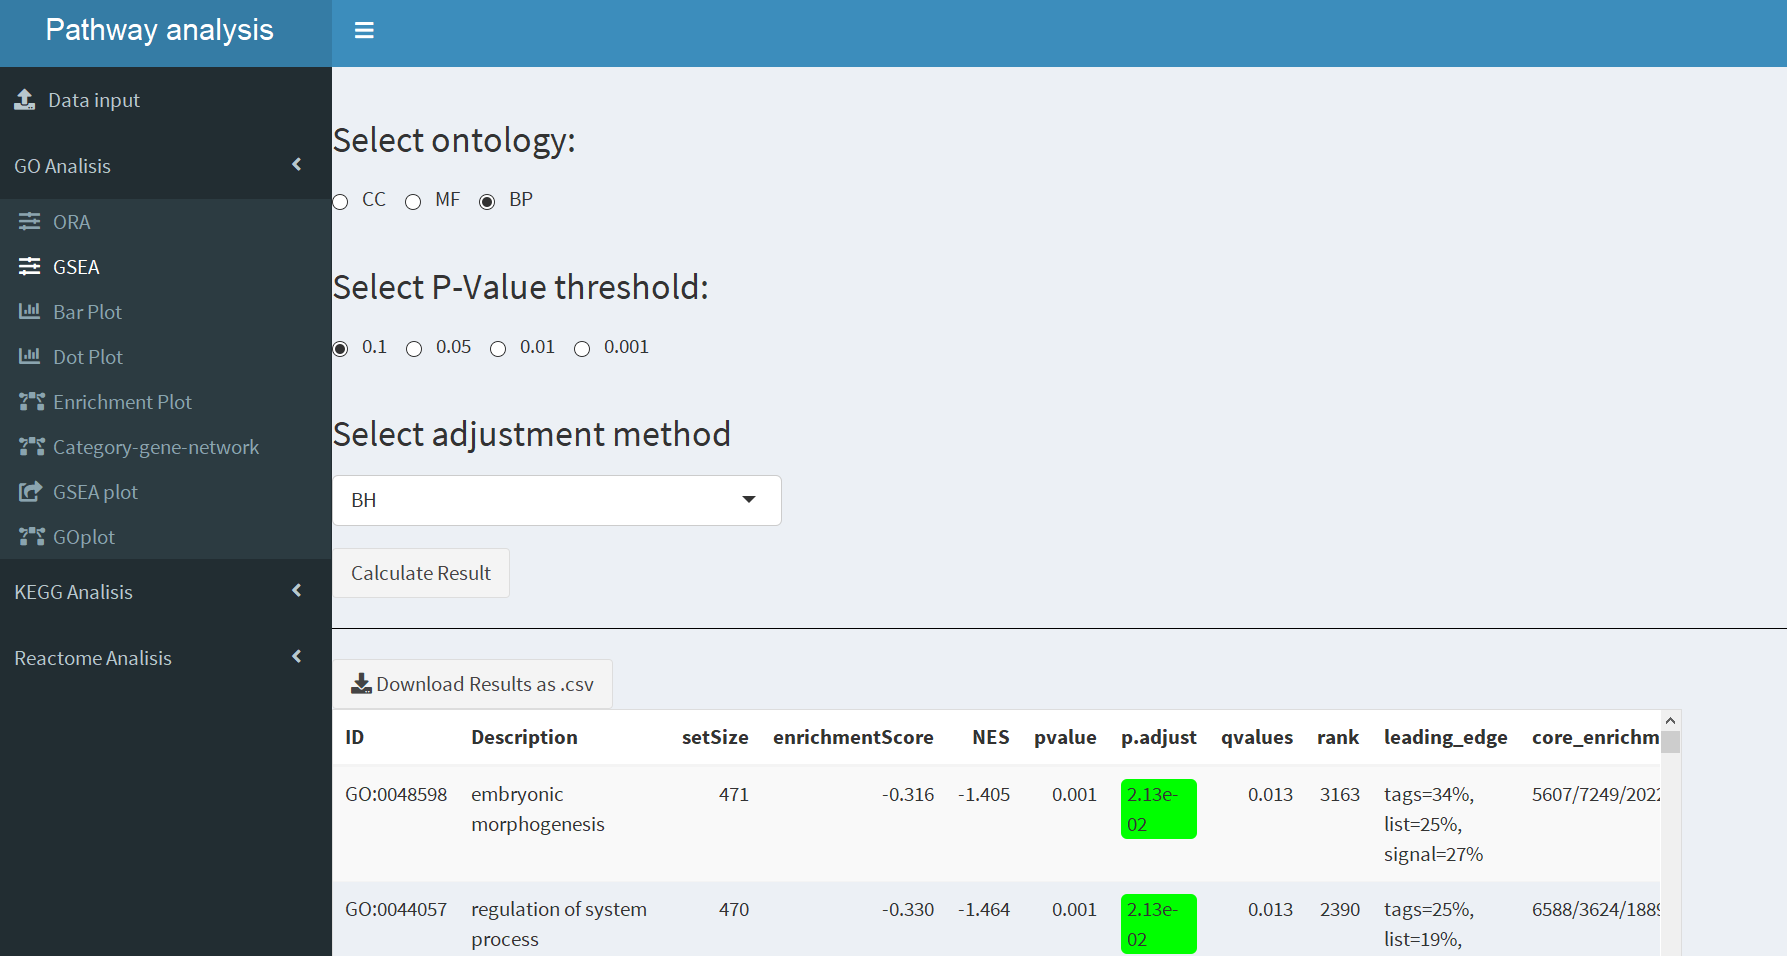
\includegraphics[width=0.9\textwidth]{App_F11_Items_GO_GSEA.png}  
\caption{El resultat d'anàlisi GSEA. GO.}
\end{figure}

\subsubsection{KEGG}
De la mateixa manera es calucula GSEA amb la funció \helvetica{gseKEGG()} del paquet \helvetica{clusterProfiler}:

\begin{figure}[H]
\centering
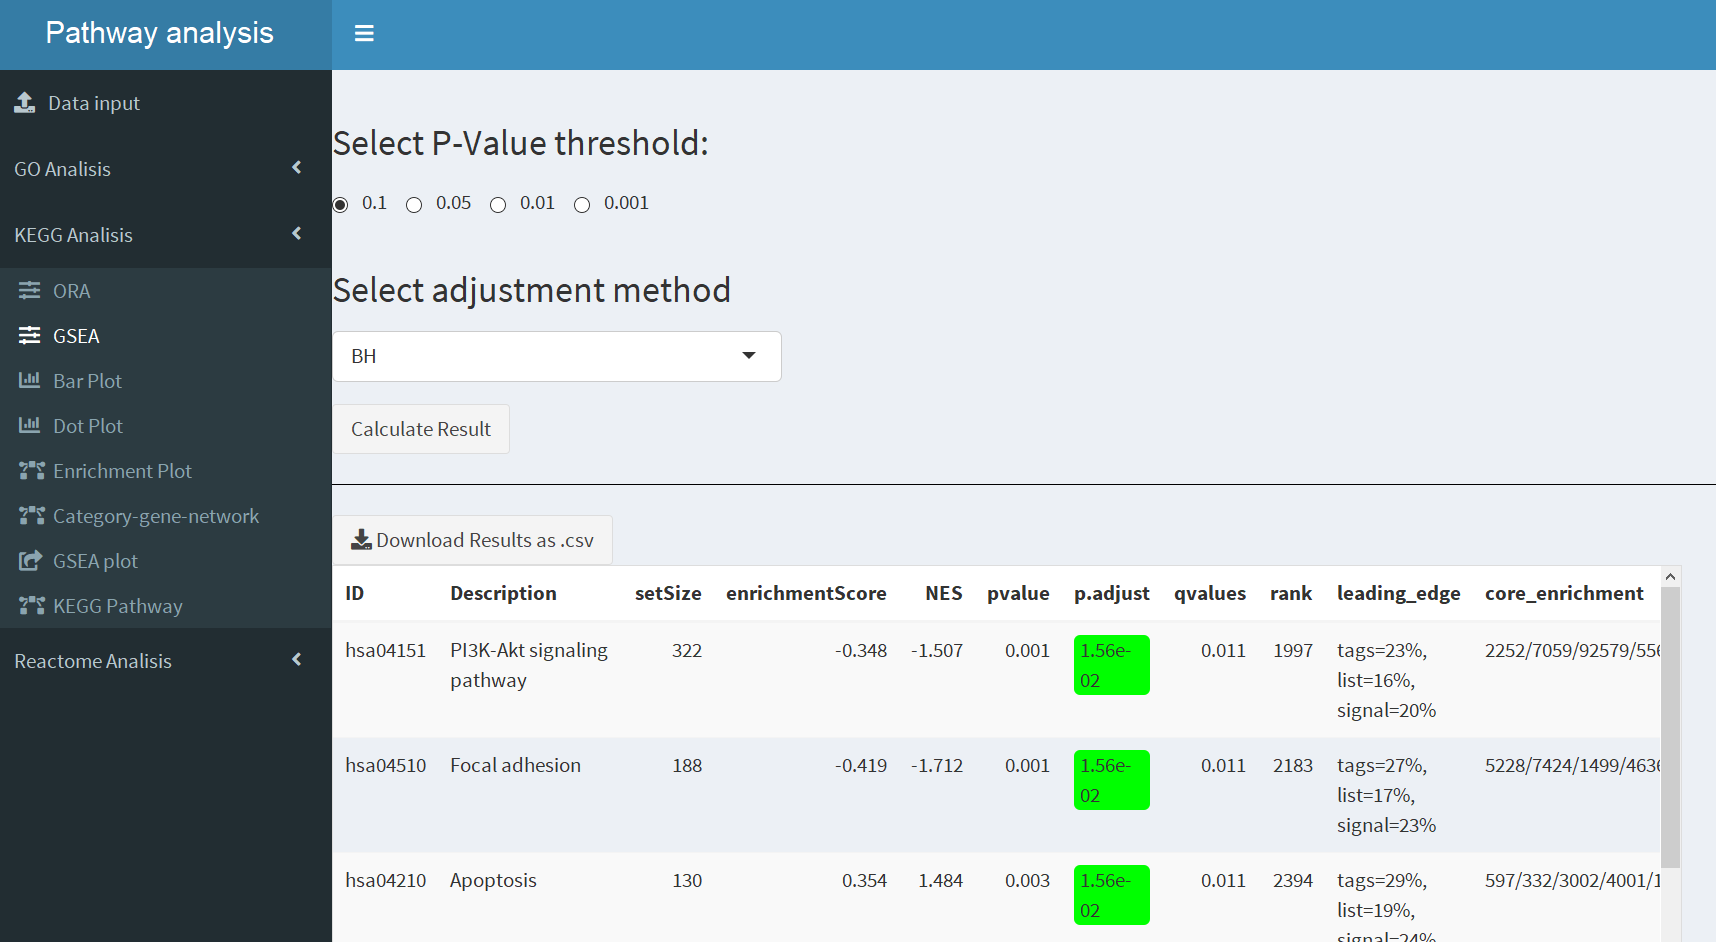
\includegraphics[width=0.9\textwidth]{App_F12_Items_KEGG_GSEA.png}  
\caption{El resultat d'anàlisi GSEA. KEGG.}
\end{figure}

\subsubsection{Reactome}
Per completar l'anàlisi l'usuari pot calcular GSEA per a base de dades Reactome. Com als altres casos utilitzo el paquet \helvetica{clusterProfiler} i específicament la funció \helvetica{gsePathway()}

\begin{figure}[H]
\centering
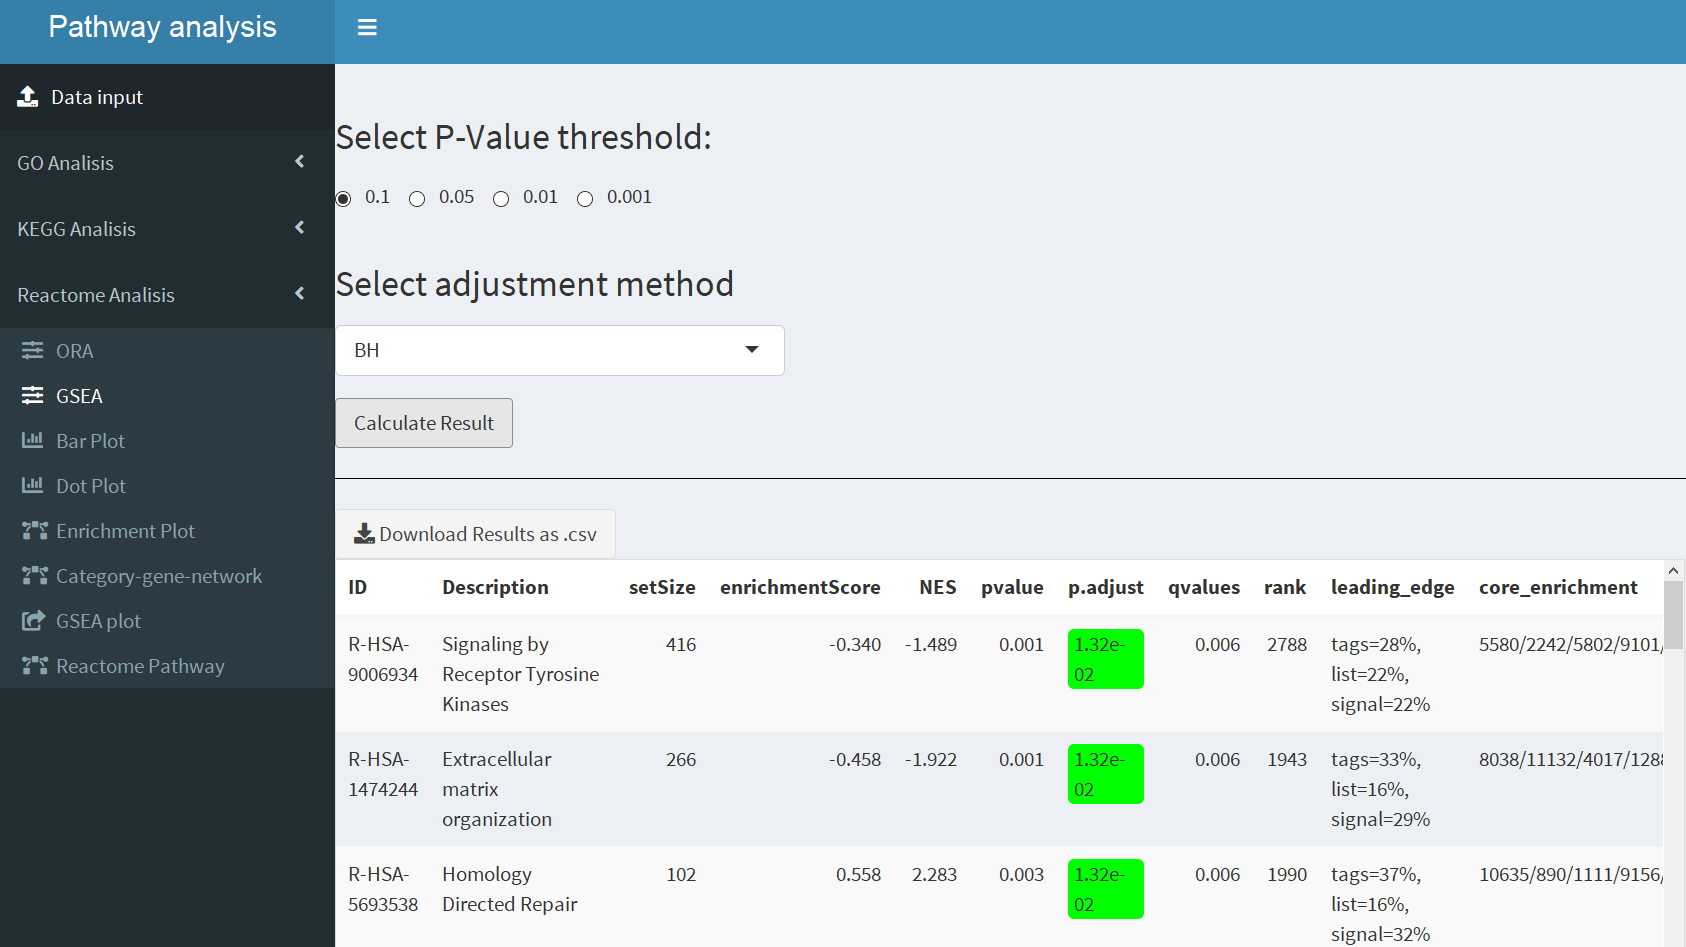
\includegraphics[width=0.9\textwidth]{App_F13_Items_RA_GSEA.png}  
\caption{El resultat d'anàlisi GSEA. Reactome.}
\end{figure}

\subsection{Bar-Plots}
Els resultats de \helvetica{enrichGO}, \helvetica{enrichKEGG} i \helvetica{enrichPathway} es pot visualitzar amb el gràfic de barres. L'usuari pot elegir el nombre de les categories visualitzades entre 2 i 30. Es dona l'opció per descargar el gràfic en format .png.

\begin{figure}[H]
\centering
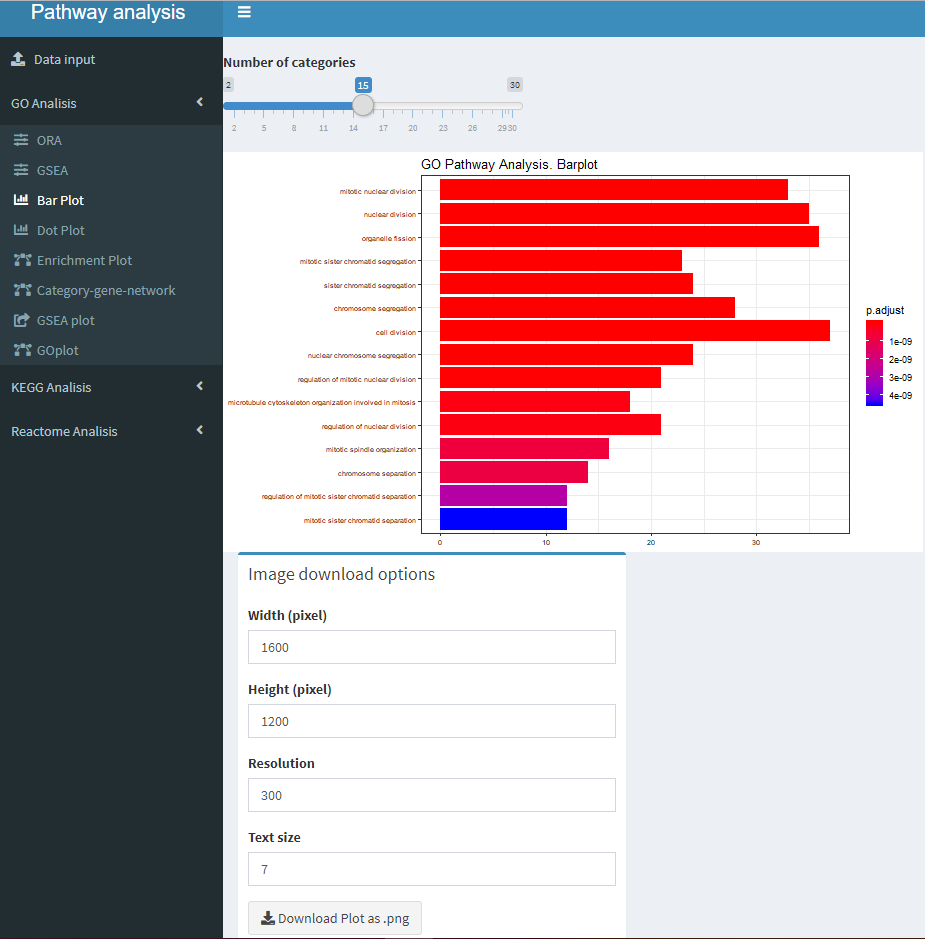
\includegraphics[width=0.9\textwidth]{App_F14_Items_GO_BarPlot.png}  
\caption{Bar-Plot. GO.}
\end{figure}

\subsection{Dot-Plots}

El \textit{dot plot} visualitza addicionalment el \textit{gen ratio}. També aquí l'usuari pot selecionar el nombre de les categories.


\begin{figure}[H]
\centering
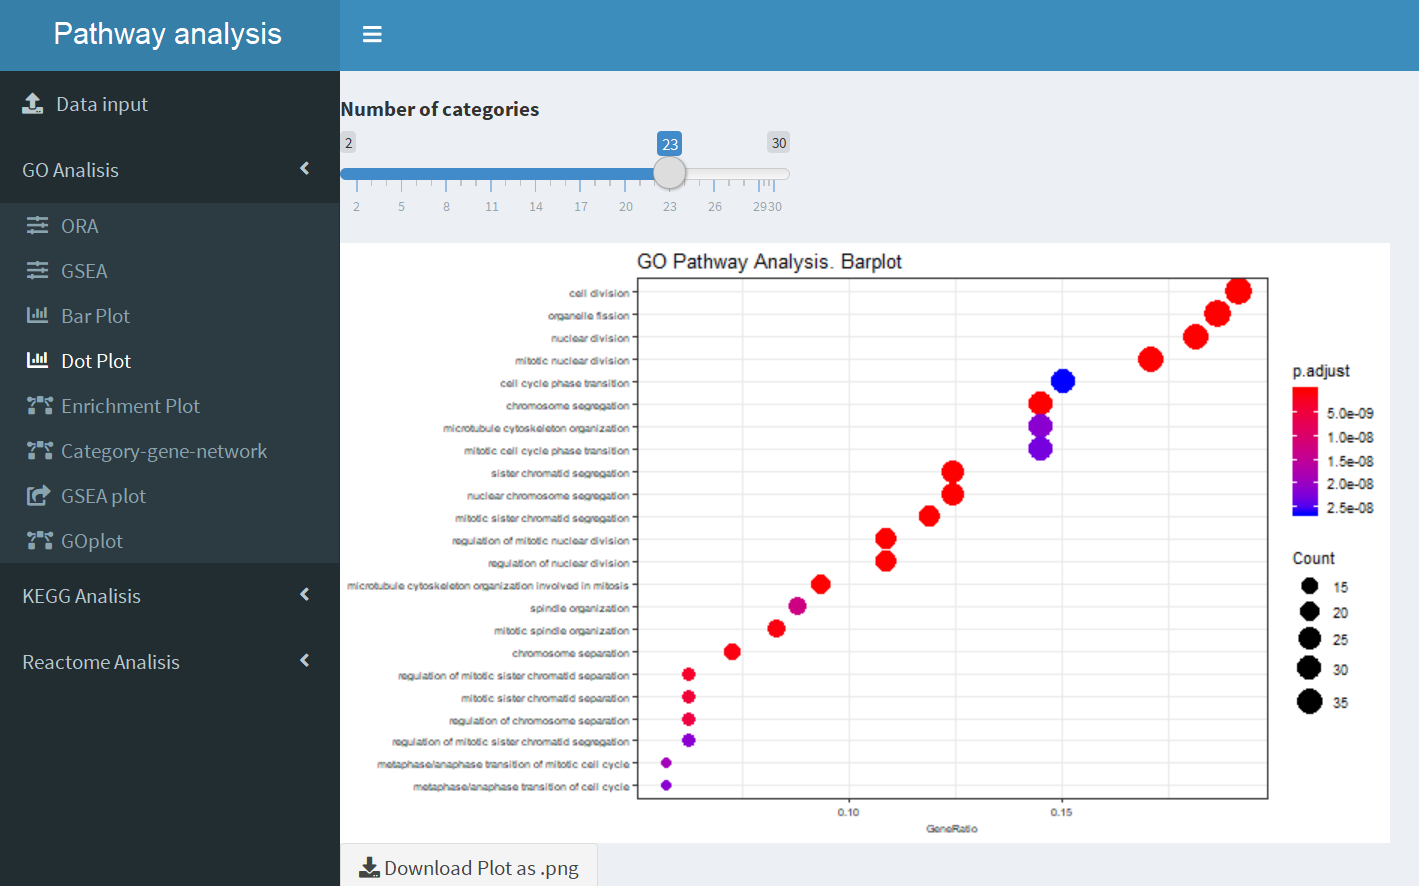
\includegraphics[width=0.9\textwidth]{App_F15_Items_GO_DotPlot.png}  
\caption{Bar-Plot. GO.}
\end{figure}

\subsection{Enrichment Plots}

\begin{figure}[H]
\centering
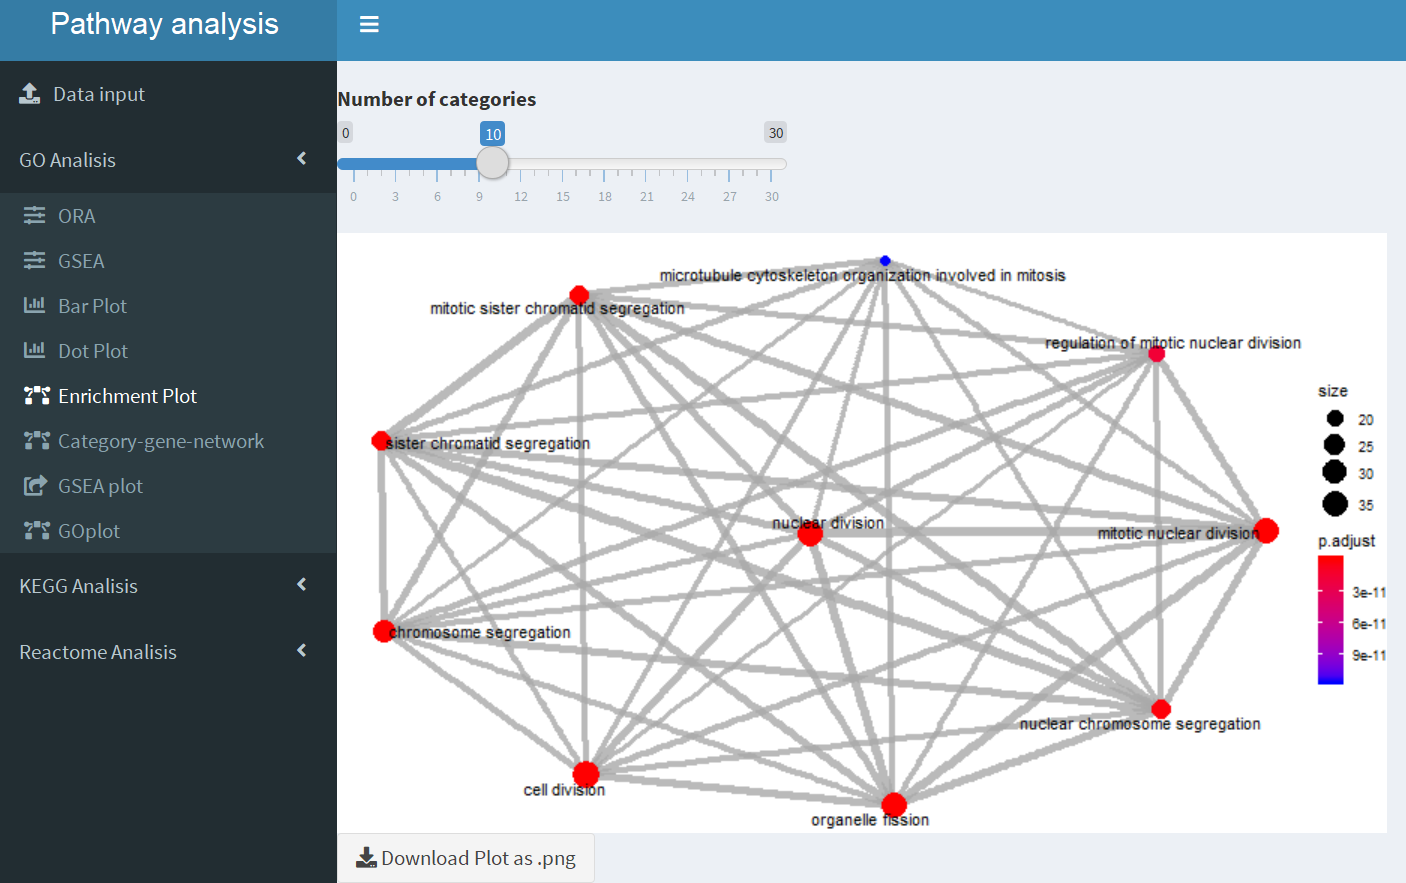
\includegraphics[width=0.9\textwidth]{App_F16_Items_GO_Emap.png}  
\caption{Bar-Plot. GO.}
\end{figure}

\subsection{Category-Gene-Network Plot}

\begin{figure}[H]
\centering
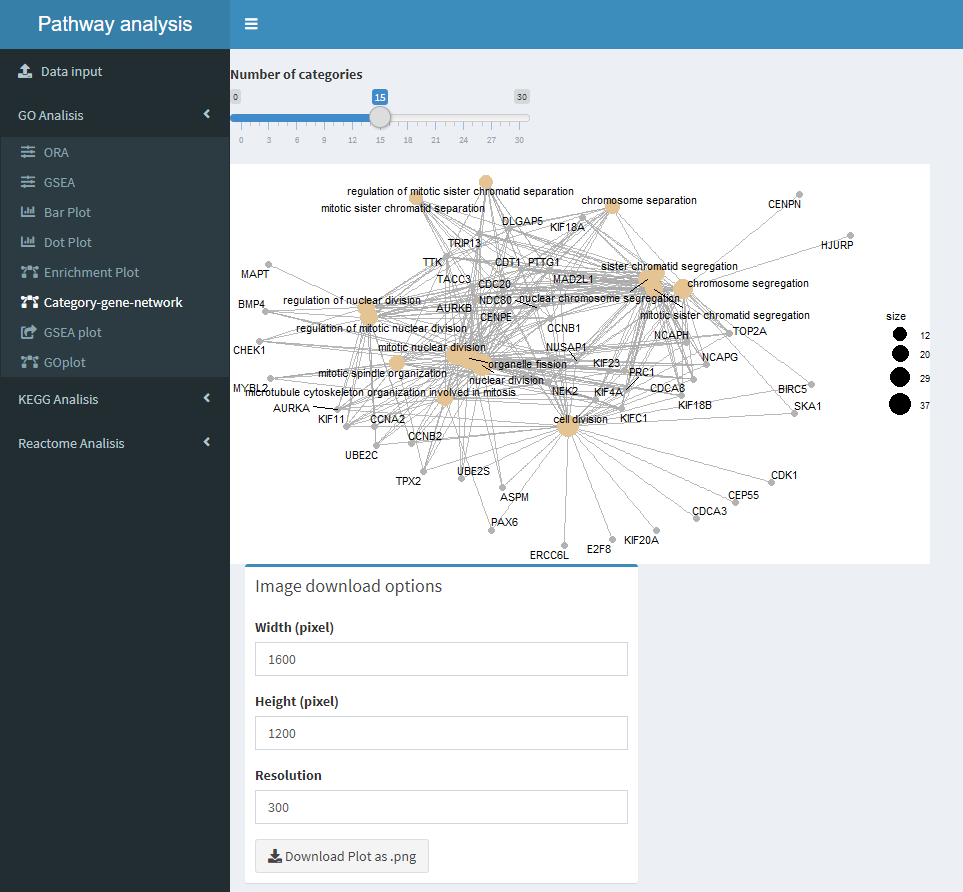
\includegraphics[width=0.9\textwidth]{App_F17_Items_GO_CnetPlot.png}  
\caption{Category-Gene-Network Plot. GO.}
\end{figure}

\subsection{GSEA Plot}
L'usuari pot visualitzar una de les categories disponibles via \textit{dropdown list}. El llistat inclou totes les rutes generades durant l'anàlisi GSEA en els apartats \textit{Go Analysis}$\rightarrow$\textit{GSEA}; \textit{KEGG}$\rightarrow$\textit{GSEA}
\begin{figure}[H]
\centering
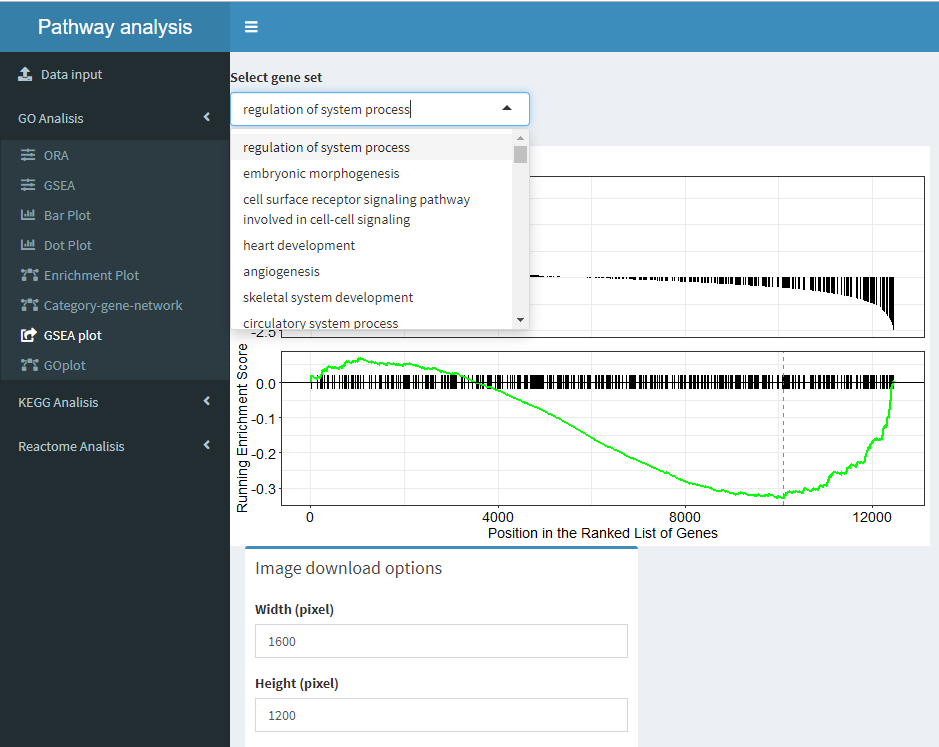
\includegraphics[width=0.9\textwidth]{App_F18_Items_GO_GSEA_Plot.png}  
\caption{GSEA Plot. GO.}
\end{figure}


\section{L'anàlisi específic de GO, KEGG i Reactome}

\subsection{GO Plot}

\begin{figure}[H]
\centering
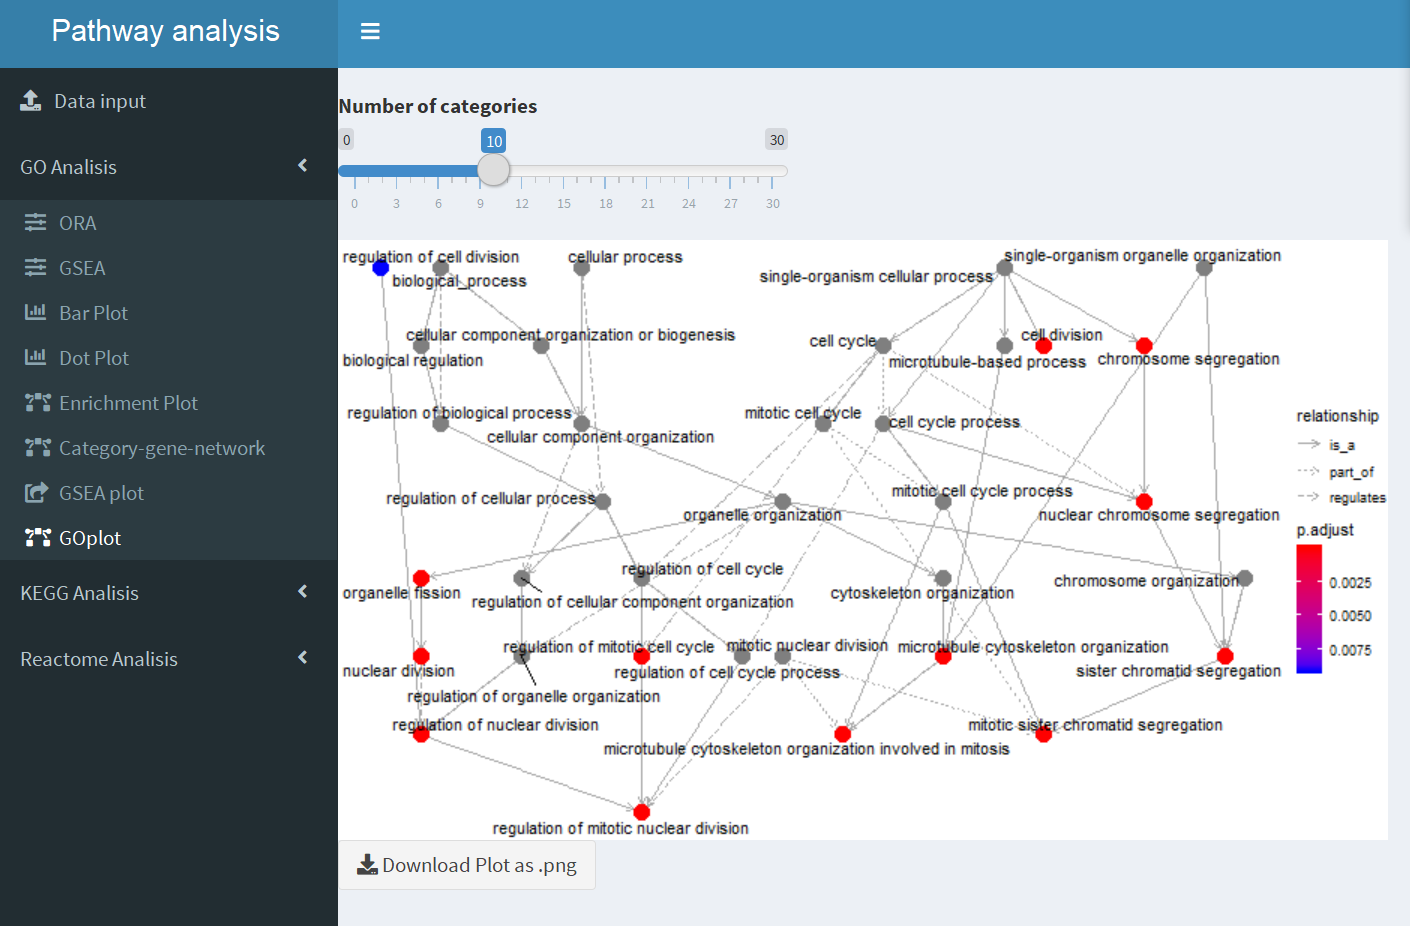
\includegraphics[width=0.9\textwidth]{App_F19_Items_GO_GOPlot.png}  
\caption{GO Plot}
\end{figure}

\subsection{KEGG Pathway}

\begin{figure}[H]
\centering
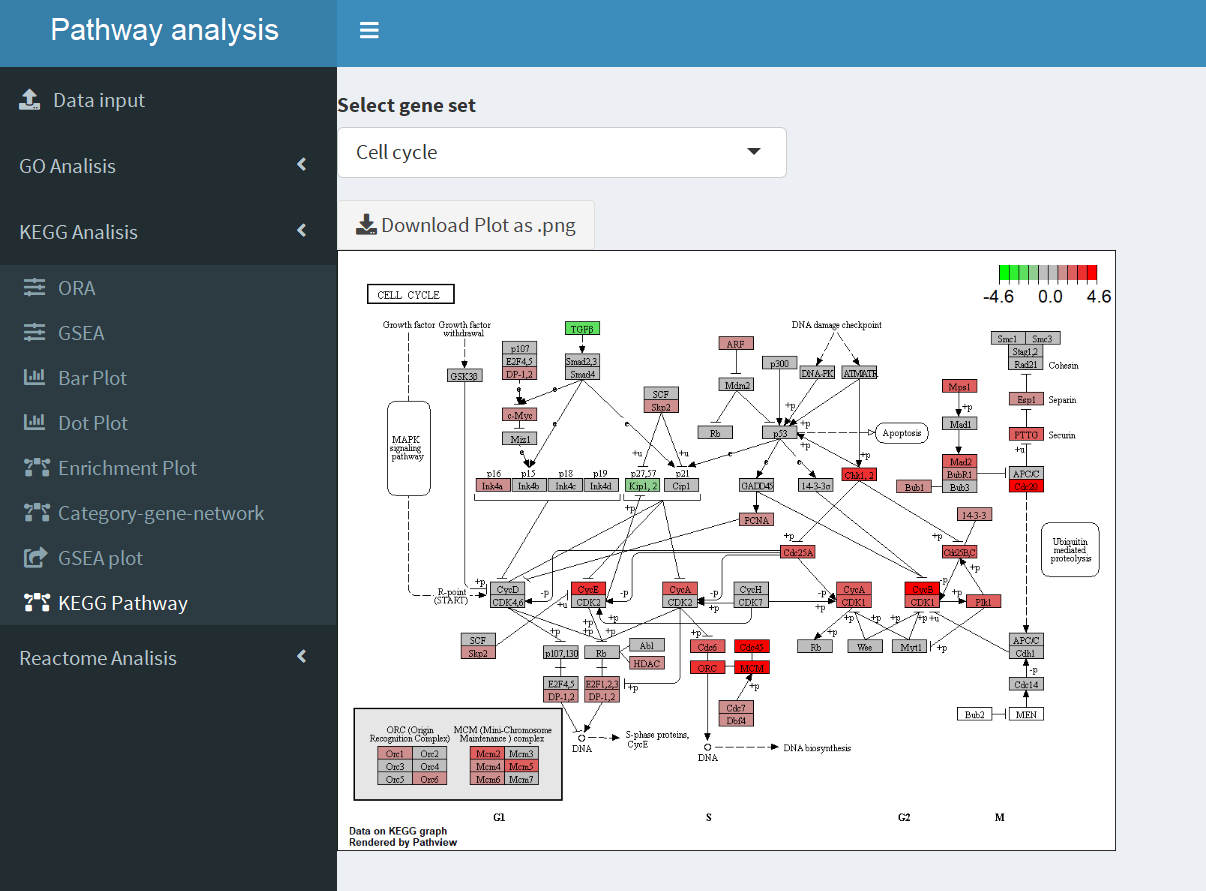
\includegraphics[width=0.9\textwidth]{App_F20_Items_KEGG_KEGGPathway.png}  
\caption{KEGG pathway}
\end{figure}

\subsection{Reactome Pathway}

\begin{figure}[H]
\centering
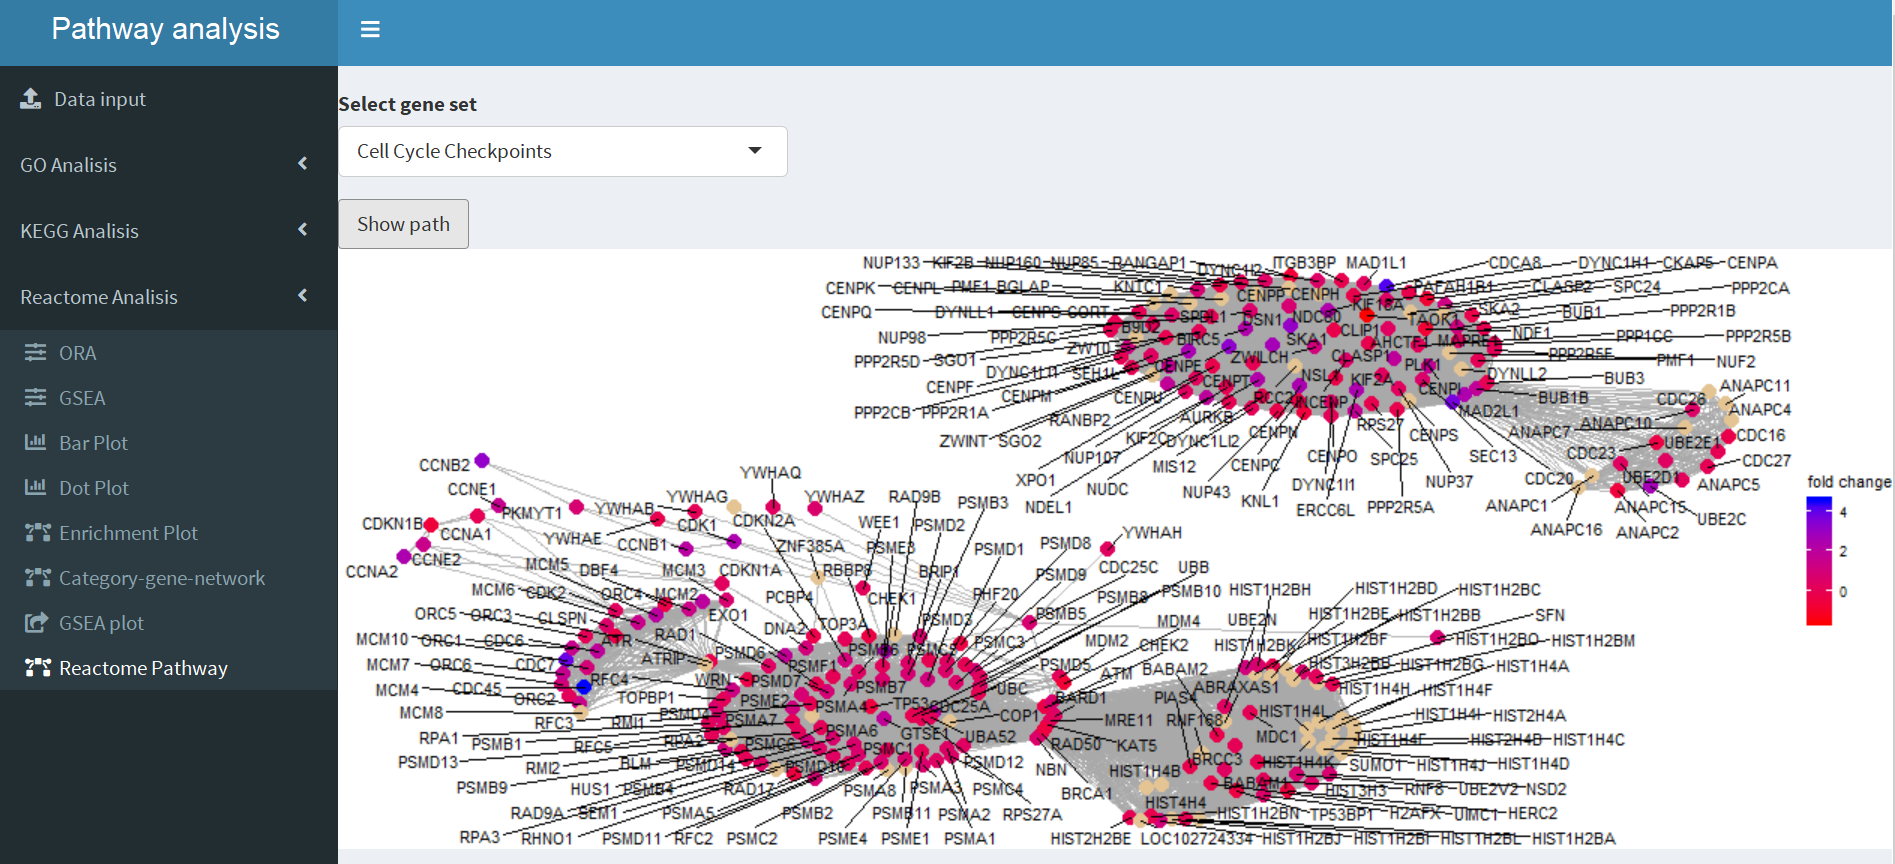
\includegraphics[width=0.9\textwidth]{App_F21_Items_RA_RAPathway.png}  
\caption{Reactome pathway}
\end{figure}


\end{document}
